
\graphicspath{{./fig_LDC112/}}

%
\subsection{直方体内のキャビティ流れ: LDC112}

\subsubsection{目的}
本例題は,辺の長さが$1:1:2$となる3次元キャビティフローの初期時間発展の問題である.Rectangular組み込み例題クラスの3次元モデルを用いて解析し,Guermond\cite{guermond:02:JFM}が行った実験およびFEMシミュレーションと比較することにより,CBCソルバーの精度を検証する.

\subsubsection{問題の定義}
辺の長さの比が$X:Y:Z=1:1:2$である直方体の,$Y$マイナス面壁を$X$マイナス方向に一定速度$U$でスライドしたときに直方体内の静止している流体に生じる三次元非定常流れである.

\subsubsection{計算領域と観測}
計算領域は,\textbf{図\ref{fig:LDC112}}に示すような直方体である.

\begin{figure}[htbp]
\centering
\includegraphics[width=12cm, bb=0 0 617 414]{LDC112.png}
\caption{計算領域の設定}
\label{fig:LDC112}
\end{figure}

$Y-$面は,$(u, v, w)=(-U, 0, 0)$のスライド壁,それ以外の$X\pm$面,$Y+$面,$Z\pm$面は,固定壁である.

流速ベクトルの観測は,$t = 4, \, 6, \,8, \,10, \,12$の無次元時刻に,$z = 0, \,0.5, \,0.75$の$xy$面内において行った.
%$Y$マイナス面以外はすべて固定壁.
%$Y$マイナス面(Lid)は$X$軸方向に無限に大きいとし,それが$X$軸マイナス方向に一定速度($U=1$)で滑ることにより誘起される(Driven),直方体(Cavity)内の流れの速度ベクトルを$z=0, \, 0.5, \, 0.75$において,$t=4, \, 6, \, 8, \, 10, \, 12$の時刻に観測した.

格子分割数は,$64\times 64 \times 128$である.

\subsubsection{計算環境}
本計算に利用した計算機環境とソフトウェアを\textbf{表\ref{tbl: LDC112 env}}に示す.

\begin{table}[htdp]
\small
\caption{計算機環境および利用ソフトウェア}
\begin{center}
\begin{tabular}{ll}\toprule
Computer & eX. COMPUTER\\
CPU & Intel Core i7-950 (4 Cores/CPU)\\
Clock & 3.07 GHz\\
Memory & 12GB \\
Cache & 8 MB\\
%Cache(3rd) & 4MB\\ 
OS & Linux ubuntu 2.6.32-25-generic\\ \hline
MPI & OpenMPI 1.4.3\\
V-Sphere & ver. 1.8.4\\
CBC & ver. 1.3.3\\
FlowBase & ver. 2.3.4\\ \hline
Compiler & Intel Compiler Composer XE(12.0) 2011.3.174 C++/Fortran\\
Compile Option & -O3\\
\bottomrule
\end{tabular}
\end{center}
\label{tbl: LDC112 env}
\end{table}

\subsubsection{解析モデルと計算パラメータ}
計算は,Guermondの実験を踏襲して,有次元のパラメータを入力して行った.
Navier-Stokes方程式を基礎方程式とし,時間積分は一次精度Euler陽解法,
解法アルゴリズムにはFractional Step法を用いた.
また,対流項の計算スキームには,三次精度MUSCLスキームを用いた.

解析モデルは,組み込み例題3次元のRectangularクラスから提供される(example.svx).

計算に用いたパラメータ(\textbf{表\ref{Table.paramLDC}}),流体の物性値(\textbf{表\ref{Table.busseiLDC}})などを示す.
\begin{table}[htbp]
\centering
\caption{計算に用いたパラメータ}
\label{Table.paramLDC}
\begin{tabular}{llll}\toprule
$h$ &短辺の長さ &$6.2\times10^{-2}$ &[m]\\
$U$ &$y=0$の壁面の移動速度 & $1.8\times10^{-2}$ &[m/s]\\
$\delta \tau $& 定速に達するまでの加速時間&$0.05$ &[s]\\
$\nu $ & クーラン数 & 0.1 & \\
\bottomrule
\end{tabular}
\end{table}

\begin{table}[htbp]
\centering
\caption{計算に用いた物性値}
\label{Table.busseiLDC}
\begin{tabular}{llll}\toprule
物性 &&物性値  & [単位]\\
\midrule
$\rho$ & 密度 & 998.2 & kg/m$^3$\\
$\mu$  & 粘性係数 & 1002.6 $\times 10^{-6}$ &[Pa $\cdot$ s]\\
\bottomrule
\end{tabular}
\end{table}

\subsubsection{サンプリングの指定}
\textbf{図\ref{fig:LDC112}}の$z=0, \, 0.5, \, 0.75$の$xy$面内において,$x=0.5, \, 0 \leq y \leq 1$の$x$方向の速度成分$u$, および$y=0.5, \, 0 \leq x \leq 1$の$y$方向の速度成分$v$を,$t=4, \, 6, \, 8, \, 10, \, 12$の無次元時刻にサンプリングした.

\subsubsection{解析結果}
計算結果のVelocity Profileを,Guermondによる実験値および有限要素法(FEM)でのシミュレーション結果と比較した.ここでは,$t=4$および$t=12$を\textbf{図\ref{fig:VP}}に示す.

Velocity Profileは,無次元で,$0.5-y$ に対する$ -0.5u$と,$0.5-x$ に対する$-0.5v$を同じ図にプロットすることにより作成している.

CBCの本解析結果は,Guermondの実験値,FEMの結果とよい一致を見せているといえる.

\begin{figure}[htdp]
\centering
\begin{minipage}{16cm}
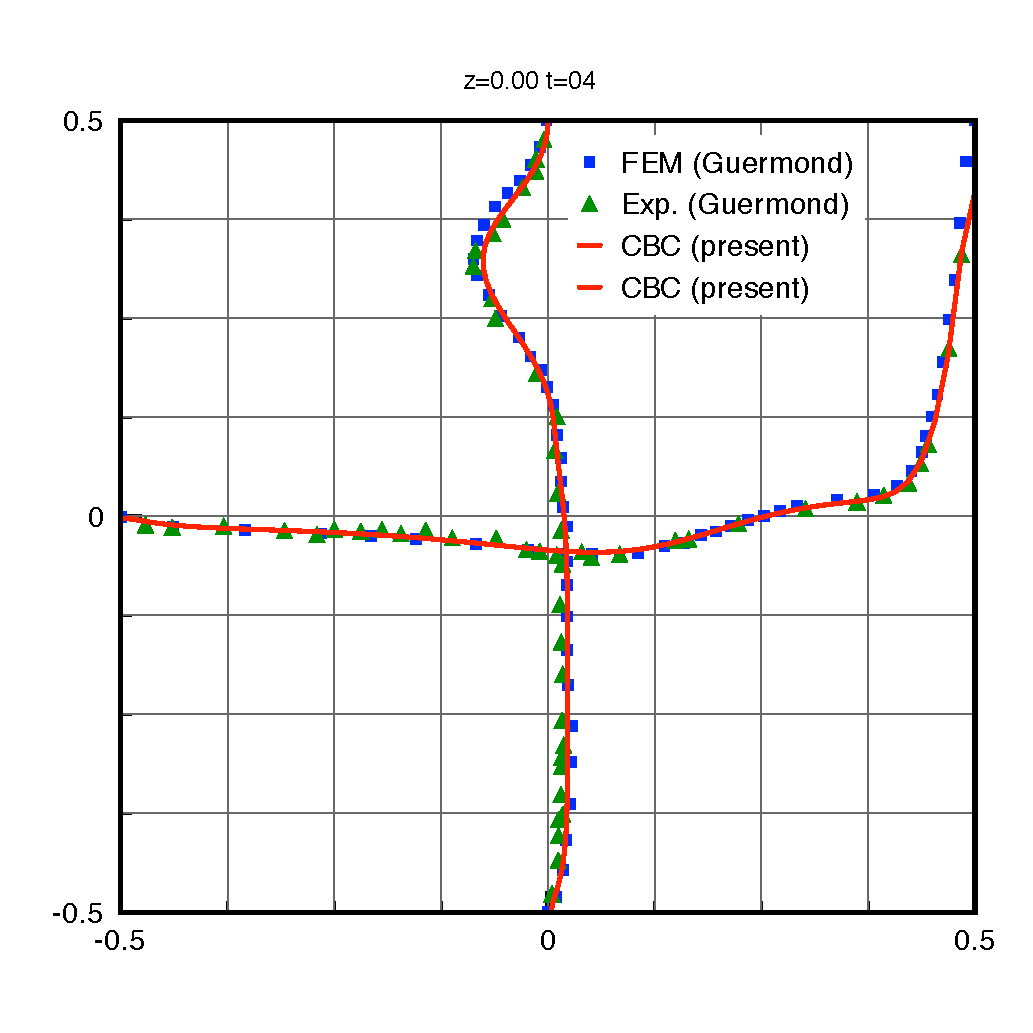
\includegraphics[width=8cm]{z00t04.eps}
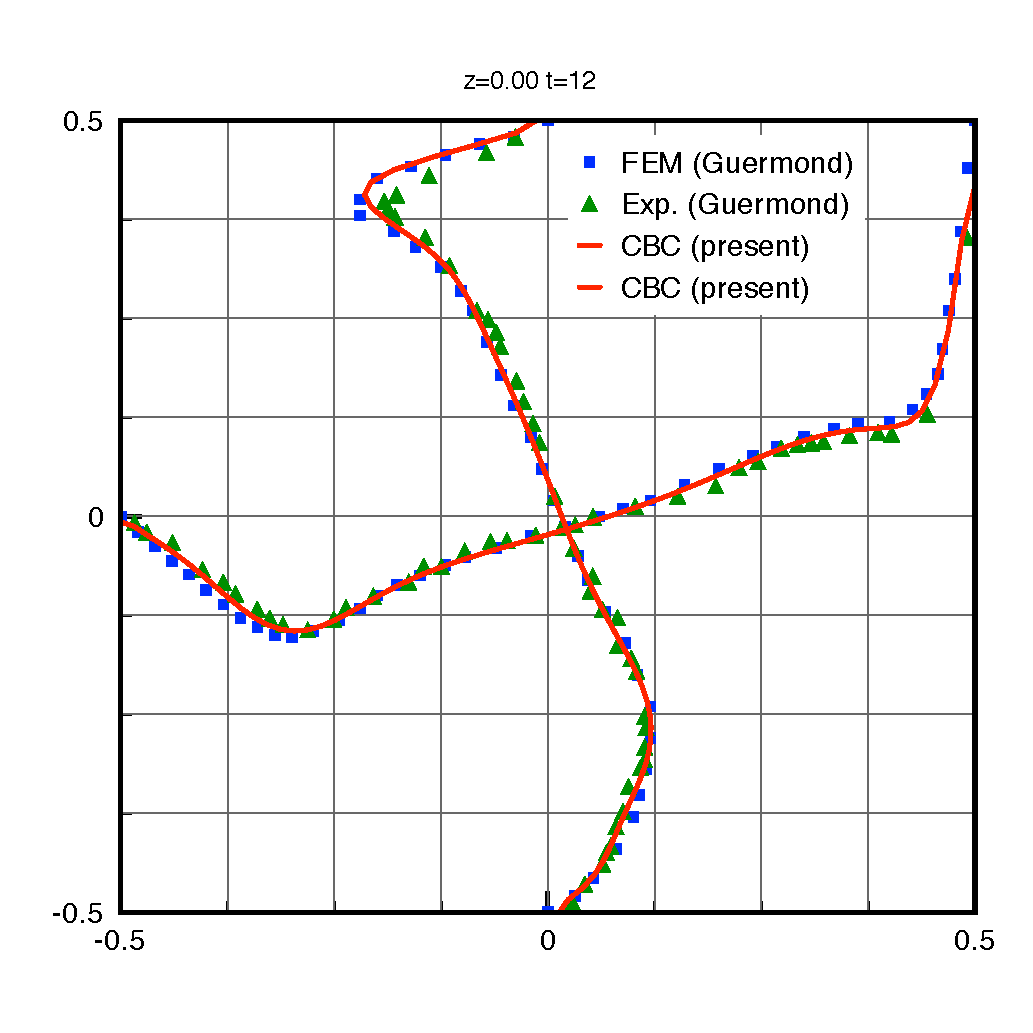
\includegraphics[width=8cm]{z00t12.eps}
\end{minipage}
\begin{minipage}{16cm}
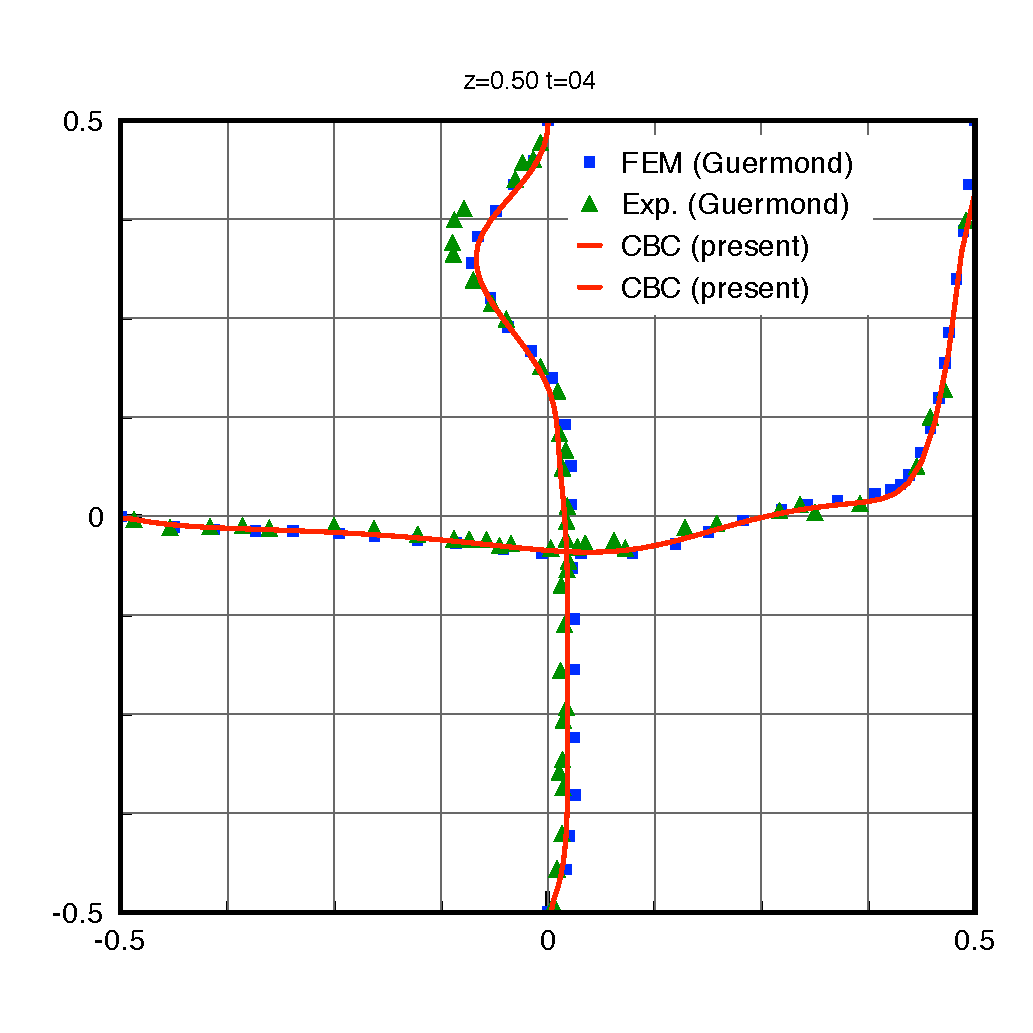
\includegraphics[width=8cm]{z50t04.eps}
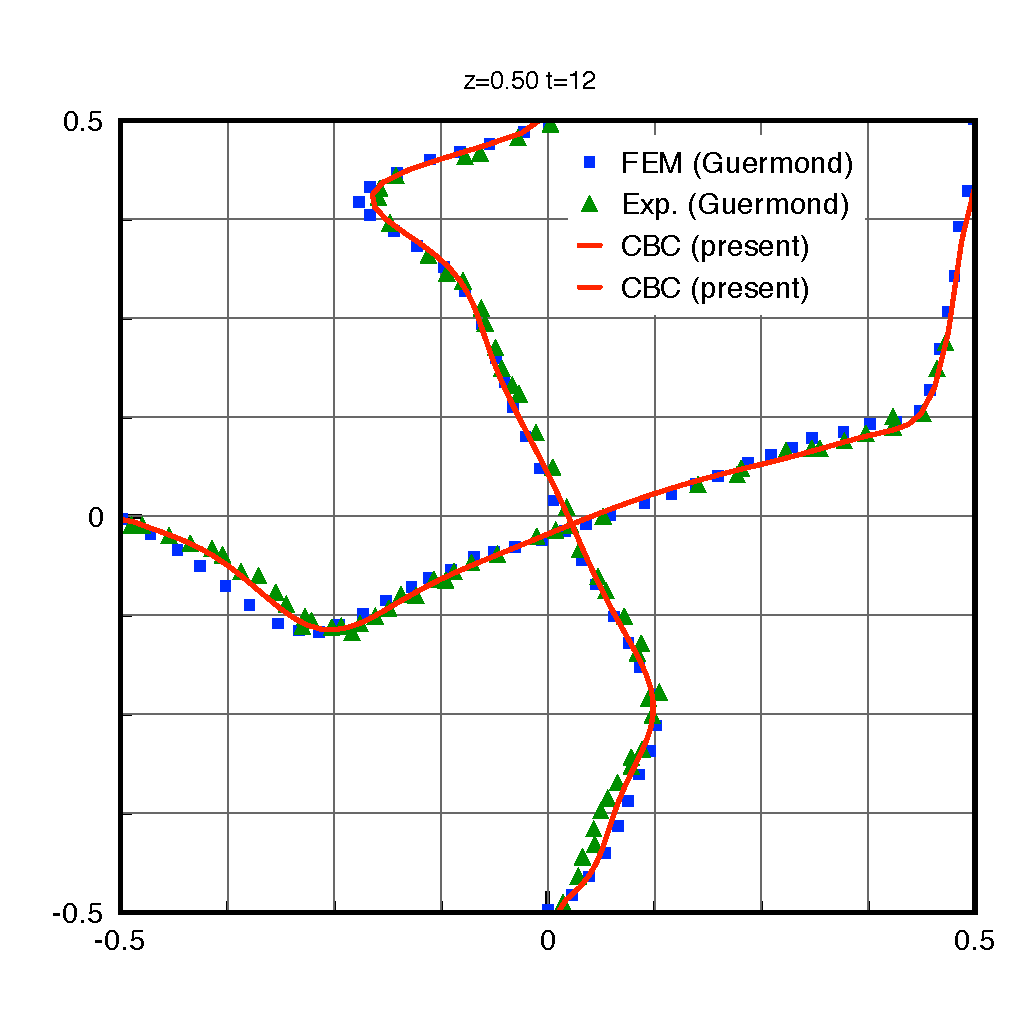
\includegraphics[width=8cm]{z50t12.eps}
\end{minipage}
\begin{minipage}{16cm}
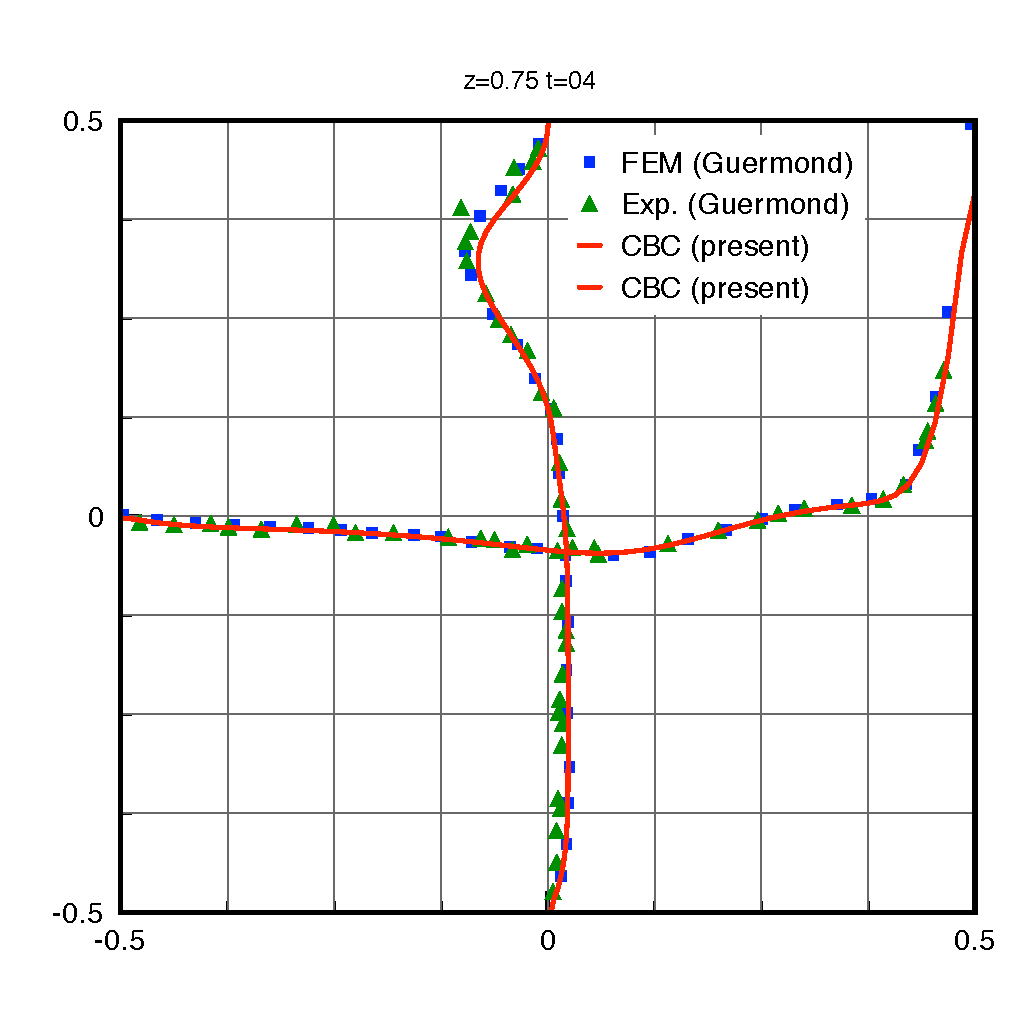
\includegraphics[width=8cm]{z75t04.eps}
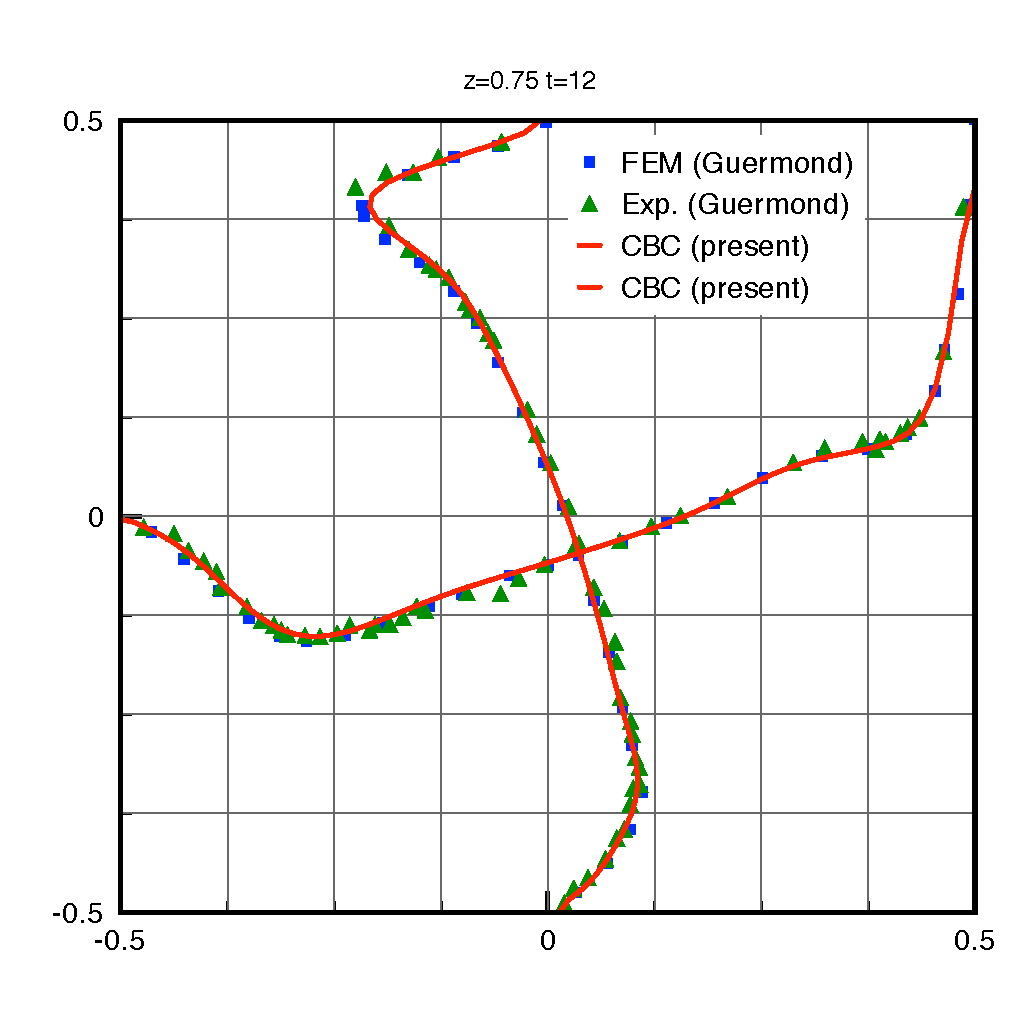
\includegraphics[width=8cm]{z75t12.eps}
\end{minipage}
\caption{$t=4$(左)と$t=12$(右)における$z=0, \, 0.5, \, 0.75$面のVelocity Profile}
\label{fig:VP}
\end{figure}

\subsubsection{ファイルのメモ}
例題の提供ファイルの説明を以下に示す.\\
\vspace{3mm}

\begin{tabularx}{180mm}{l@{}c@{}l@{}c@{}lX}
example\CID{07480}LDC112\, & \CID{07530}&\CID{00718}&\CID{07530}&sample\_\CID{00718}\_x.log & \CID{00718}($z=0,\,0.5,\,0.75$)の場合の$x$軸に沿ったsamplingファイル\\
&\CID{07482}&&\CID{07514}&sample\_\CID{00718}\_y.log & \CID{00718}($z=0,\,0.5,\,0.75$)の場合の$y$軸に沿ったsamplingファイル\\
&\CID{07482}&&\CID{07502}&\CID{00718}\CID{00734}.plot & \CID{00718}($z$情報), \CID{00734}($t$情報)のplotファイル(\url{http://plot.micw.eu/})\\
&\CID{07514}&\multicolumn{3}{l}{condition.txt} & conditionファイル\\
&\CID{07514}&\multicolumn{3}{l}{DomainInfo.txt} & 計算領域情報ファイル\\
&\CID{07514}&\multicolumn{3}{l}{example.svx.zip} & 出力された解析モデル圧縮ファイル\\
&\CID{07514}&\multicolumn{3}{l}{history\_base.log} & 履歴ファイル\\
&\CID{07514}&\multicolumn{3}{l}{ldc.xml} & コンフィギュレーションXMLファイル\\
&\CID{07502}&\multicolumn{3}{l}{profiling.txt} & 実行時性能測定結果ファイル
\end{tabularx}
